\documentclass[11pt]{article}
\usepackage[margin=1in]{geometry}
\usepackage{amsmath, amssymb, amsthm}
\usepackage{graphicx}
\usepackage{tikz}
\usetikzlibrary{arrows.meta, positioning, automata, calc, decorations.markings}

% Colors
\definecolor{garnet}{HTML}{73000A}

% Paragraph formatting - no indentation, extra spacing
\setlength{\parindent}{0pt}
\setlength{\parskip}{1em}

% Theorem environments
\theoremstyle{definition}
\newtheorem{definition}{Definition}
\newtheorem{example}{Example}
\newtheorem{remark}{Remark}

\title{\textcolor{garnet}{\textbf{Markov Reward Processes: Computing State Values}}}
\author{J.C. Vaught}
\date{\vspace{-2em}}

\begin{document}
\maketitle

\section{Introduction}

A \textbf{Markov Reward Process (MRP)} extends a standard Markov chain by associating a reward with each state. This framework is fundamental in reinforcement learning, economics, and operations research, where we want to evaluate the long-term value of being in a particular state.

\begin{definition}[Markov Reward Process]
A Markov Reward Process is a tuple $\langle \mathcal{S}, \mathcal{P}, \mathcal{R}, \gamma \rangle$ where:

\begin{center}
\begin{tabular}{c l l}
\hline
\textbf{Symbol} & \textbf{Name} & \textbf{Description} \\
\hline
$\mathcal{S}$ & State space & Finite set of states \\
$\mathcal{P}$ & Transition matrix & $\mathcal{P}_{ss'} = P(S_{t+1} = s' \mid S_t = s)$ \\
$\mathcal{R}$ & Reward function & $\mathcal{R}_s = \mathbb{E}[R_{t+1} \mid S_t = s]$ \\
$\gamma$ & Discount factor & $\gamma \in [0, 1]$ \\
\hline
\end{tabular}
\end{center}
\end{definition}

\section{Problem Setup}

Consider the following three-state Markov Reward Process:

\begin{center}
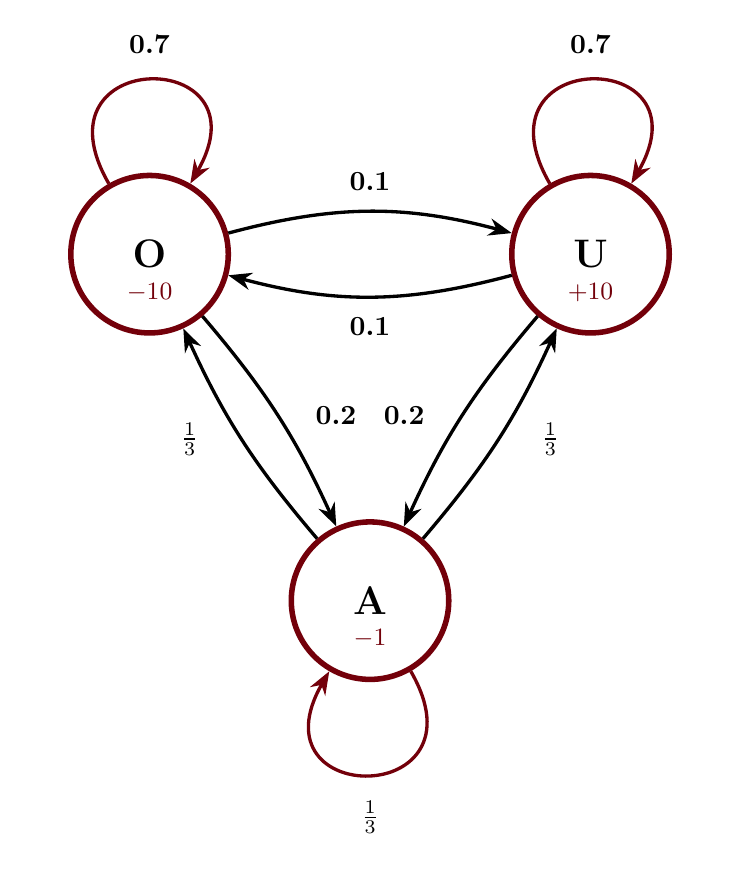
\begin{tikzpicture}[
    >=Stealth,
    scale=0.8,
    every state/.style={
        fill=white,
        draw=garnet,
        line width=2pt,
        text=black,
        minimum size=2cm,
        font=\bfseries\Large
    },
    every edge/.style={
        draw=black,
        line width=1.2pt,
        ->,
        >=Stealth
    },
    prob/.style={
        font=\bfseries,
        text=black,
        fill=white,
        inner sep=3pt
    },
    statelabel/.style={
        font=\small\bfseries,
        text=garnet
    }
]

% States
\node[state] (O) at (0, 0) {O};
\node[statelabel, below=1pt of O.center, yshift=-6pt] {$-10$};

\node[state] (U) at (7, 0) {U};
\node[statelabel, below=1pt of U.center, yshift=-6pt] {$+10$};

\node[state] (A) at (3.5, -5.5) {A};
\node[statelabel, below=1pt of A.center, yshift=-6pt] {$-1$};

% Self-loops
\path (O) edge[loop above, looseness=5, out=120, in=60, draw=garnet] node[prob, above=6pt] {0.7} (O);
\path (U) edge[loop above, looseness=5, out=120, in=60, draw=garnet] node[prob, above=6pt] {0.7} (U);
\path (A) edge[loop below, looseness=5, out=-60, in=-120, draw=garnet] node[prob, below=6pt] {$\frac{1}{3}$} (A);

% O <-> U transitions
\path (O) edge[bend left=15] node[prob, above=4pt] {0.1} (U);
\path (U) edge[bend left=15] node[prob, below=4pt] {0.1} (O);

% O <-> A transitions
\path (O) edge[bend left=8] node[prob, right=10pt, pos=0.5] {0.2} (A);
\path (A) edge[bend left=8] node[prob, left=12pt, pos=0.5] {$\frac{1}{3}$} (O);

% U <-> A transitions
\path (U) edge[bend right=8] node[prob, left=10pt, pos=0.5] {0.2} (A);
\path (A) edge[bend right=8] node[prob, right=12pt, pos=0.5] {$\frac{1}{3}$} (U);

\end{tikzpicture}
\end{center}

\subsection{State Space and Rewards}

The state space is $\mathcal{S} = \{O, U, A\}$ with immediate rewards:

\begin{center}
\begin{tabular}{c l c l}
\hline
\textbf{State} & \textbf{Name} & \textbf{Reward} & \textbf{Interpretation} \\
\hline
$O$ & Overweight & $-10$ & Penalty \\
$U$ & Underweight & $+10$ & Reward \\
$A$ & Average & $-1$ & Small penalty \\
\hline
\end{tabular}
\end{center}

\subsection{Transition Probability Matrix}

The transition dynamics are captured by the matrix $\mathcal{P}$:
\[
\mathcal{P} = \begin{pmatrix}
P(O|O) & P(U|O) & P(A|O) \\
P(O|U) & P(U|U) & P(A|U) \\
P(O|A) & P(U|A) & P(A|A)
\end{pmatrix}
= \begin{pmatrix}
0.7 & 0.1 & 0.2 \\
0.1 & 0.7 & 0.2 \\
\frac{1}{3} & \frac{1}{3} & \frac{1}{3}
\end{pmatrix}
\]

Note that each row sums to 1, as required for a valid probability distribution.

\section{The Value Function}

\begin{definition}[State Value Function]
The \textbf{value} of a state $s$ is the expected cumulative discounted reward starting from state $s$:
\[
V(s) = \mathbb{E}\left[ \sum_{t=0}^{\infty} \gamma^t R_{t+1} \;\Big|\; S_0 = s \right]
\]
\end{definition}

The discount factor $\gamma$ determines how much we value future rewards:

\begin{center}
\begin{tabular}{c l}
\hline
\textbf{Value} & \textbf{Meaning} \\
\hline
$\gamma = 0$ & Only immediate rewards matter \\
$\gamma = 1$ & Future rewards equally valuable (may diverge) \\
$\gamma \in (0,1)$ & Geometrically decreasing weight on future \\
\hline
\end{tabular}
\end{center}

\subsection{The Bellman Equation}

The value function satisfies a recursive relationship known as the \textbf{Bellman equation}. In lecture, this was presented in its compact expectation form:
\[
V(s) = R(s) + \gamma \, \mathbb{E}\big[V(S_{t+1}) \mid S_t = s\big]
\]

While one could derive the value function using the formulation provided in class, I found it to be unwieldy and unfriendly to beginners. The expectation notation, though mathematically elegant, obscures the actual computation required. Therefore, I am utilizing the \textbf{expanded summation form}:

\[
\boxed{V(s) = R(s) + \gamma \sum_{s' \in \mathcal{S}} P(s'|s) \cdot V(s')}
\]

where:

\begin{center}
\begin{tabular}{c l}
\hline
\textbf{Symbol} & \textbf{Meaning} \\
\hline
$V(s)$ & Value of state $s$ (what we want to compute) \\
$R(s)$ & Immediate reward received in state $s$ \\
$\gamma$ & Discount factor (how much we care about future) \\
$s'$ & Each possible next state \\
$P(s'|s)$ & Probability of transitioning from $s$ to $s'$ \\
$V(s')$ & Value of the next state $s'$ \\
\hline
\end{tabular}
\end{center}

\begin{remark}[Equivalence of Forms]
These two forms are mathematically identical. The expectation $\mathbb{E}[V(S_{t+1}) | S_t = s]$ is simply the probability-weighted sum over all possible next states:
\[
\mathbb{E}\big[V(S_{t+1}) \mid S_t = s\big] = \sum_{s' \in \mathcal{S}} P(s'|s) \cdot V(s')
\]
The expanded form makes explicit \textit{how} to actually compute the expectation, which is far more useful when solving problems by hand.
\end{remark}

This equation states that the value of a state equals:
\begin{enumerate}
    \item The \textbf{immediate reward} $R(s)$, plus
    \item The \textbf{discounted expected value} of the next state (summing over all possibilities)
\end{enumerate}

\section{Hand Derivation}

Let us solve for $V(O)$, $V(U)$, and $V(A)$ with discount factor $\gamma = 0.9$.

\subsection{Step 1: Write the Bellman Equations}

Applying the Bellman equation to each state:

\begin{align}
V(O) &= R(O) + \gamma \Big[ P(O|O) \cdot V(O) + P(U|O) \cdot V(U) + P(A|O) \cdot V(A) \Big] \nonumber \\
&= -10 + 0.9 \Big[ 0.7 \cdot V(O) + 0.1 \cdot V(U) + 0.2 \cdot V(A) \Big] \label{eq:vo}
\end{align}

\begin{align}
V(U) &= R(U) + \gamma \Big[ P(O|U) \cdot V(O) + P(U|U) \cdot V(U) + P(A|U) \cdot V(A) \Big] \nonumber \\
&= +10 + 0.9 \Big[ 0.1 \cdot V(O) + 0.7 \cdot V(U) + 0.2 \cdot V(A) \Big] \label{eq:vu}
\end{align}

\begin{align}
V(A) &= R(A) + \gamma \Big[ P(O|A) \cdot V(O) + P(U|A) \cdot V(U) + P(A|A) \cdot V(A) \Big] \nonumber \\
&= -1 + 0.9 \Big[ \tfrac{1}{3} \cdot V(O) + \tfrac{1}{3} \cdot V(U) + \tfrac{1}{3} \cdot V(A) \Big] \label{eq:va}
\end{align}

Notice how the expanded form makes it immediately clear what to plug in---no mysterious expectations, just probabilities and values.

\subsection{Step 2: Rearrange to Standard Form}

Expanding and collecting terms:

\textbf{From equation~\eqref{eq:vo}:}
\begin{align*}
V(O) &= -10 + 0.63 \cdot V(O) + 0.09 \cdot V(U) + 0.18 \cdot V(A) \\
V(O) - 0.63 \cdot V(O) &= -10 + 0.09 \cdot V(U) + 0.18 \cdot V(A) \\
0.37 \cdot V(O) &= -10 + 0.09 \cdot V(U) + 0.18 \cdot V(A)
\end{align*}

\textbf{From equation~\eqref{eq:vu}:}
\begin{align*}
V(U) &= 10 + 0.09 \cdot V(O) + 0.63 \cdot V(U) + 0.18 \cdot V(A) \\
0.37 \cdot V(U) &= 10 + 0.09 \cdot V(O) + 0.18 \cdot V(A)
\end{align*}

\textbf{From equation~\eqref{eq:va}:}
\begin{align*}
V(A) &= -1 + 0.3 \cdot V(O) + 0.3 \cdot V(U) + 0.3 \cdot V(A) \\
0.7 \cdot V(A) &= -1 + 0.3 \cdot V(O) + 0.3 \cdot V(U)
\end{align*}

\subsection{Step 3: Matrix Formulation}

The system can be written in matrix form as:
\[
\mathbf{V} = \mathbf{R} + \gamma \mathcal{P} \mathbf{V}
\]

Rearranging:
\[
(\mathbf{I} - \gamma \mathcal{P}) \mathbf{V} = \mathbf{R}
\]

Therefore:
\[
\boxed{\mathbf{V} = (\mathbf{I} - \gamma \mathcal{P})^{-1} \mathbf{R}}
\]

Let us compute $\mathbf{I} - \gamma \mathcal{P}$:
\[
\mathbf{I} - 0.9 \mathcal{P} =
\begin{pmatrix} 1 & 0 & 0 \\ 0 & 1 & 0 \\ 0 & 0 & 1 \end{pmatrix}
- 0.9 \begin{pmatrix} 0.7 & 0.1 & 0.2 \\ 0.1 & 0.7 & 0.2 \\ \frac{1}{3} & \frac{1}{3} & \frac{1}{3} \end{pmatrix}
\]

\[
= \begin{pmatrix}
0.37 & -0.09 & -0.18 \\
-0.09 & 0.37 & -0.18 \\
-0.3 & -0.3 & 0.7
\end{pmatrix}
\]

\subsection{Step 4: Solve the System}

Computing the inverse and multiplying by $\mathbf{R} = (-10, 10, -1)^T$:

Using Cramer's rule or matrix inversion, we obtain:
\[
\boxed{
\begin{aligned}
V(O) &\approx -23.75 \\
V(U) &\approx +32.01 \\
V(A) &\approx +1.04
\end{aligned}
}
\]

\subsection{Step 5: Interpretation}

\begin{itemize}
    \item \textbf{$V(O) \approx -23.75$}: Starting in state O is bad. The immediate reward is $-10$, and the system tends to stay in O (70\% self-loop), accumulating more negative rewards.

    \item \textbf{$V(U) \approx +32.01$}: Starting in state U is highly valuable. The immediate reward is $+10$, and the system tends to stay in U, accumulating positive rewards.

    \item \textbf{$V(A) \approx +1.04$}: Starting in state A is slightly positive. Despite the $-1$ immediate reward, there's a $\frac{1}{3}$ chance of transitioning to the valuable state U.
\end{itemize}

\section{Solution Algorithms}

\subsection{Method 1: Direct Solution (Matrix Inversion)}

For small state spaces, we can directly compute:
\[
\mathbf{V} = (\mathbf{I} - \gamma \mathcal{P})^{-1} \mathbf{R}
\]

\begin{center}
\fbox{\parbox{0.9\textwidth}{
\textbf{Algorithm 1: Direct Solution via Matrix Inversion}
\vspace{6pt}

\textbf{Input:} Transition matrix $\mathcal{P}$, reward vector $\mathbf{R}$, discount factor $\gamma$

\textbf{Output:} Value function $\mathbf{V}$
\vspace{6pt}

\begin{tabular}{ll}
1: & $\mathbf{A} \gets \mathbf{I} - \gamma \mathcal{P}$ \hfill \textit{// Compute coefficient matrix} \\
2: & $\mathbf{V} \gets \mathbf{A}^{-1} \mathbf{R}$ \hfill \textit{// Solve linear system} \\
3: & \textbf{return} $\mathbf{V}$
\end{tabular}
}}
\end{center}

\textbf{Complexity:} $O(n^3)$ for $n$ states (matrix inversion).

\subsection{Method 2: Iterative Policy Evaluation}

For large state spaces, iterative methods are more practical:

\begin{center}
\fbox{\parbox{0.9\textwidth}{
\textbf{Algorithm 2: Iterative Policy Evaluation}
\vspace{6pt}

\textbf{Input:} Transition matrix $\mathcal{P}$, reward vector $\mathbf{R}$, discount factor $\gamma$, threshold $\theta$

\textbf{Output:} Value function $\mathbf{V}$
\vspace{6pt}

\begin{tabular}{ll}
1: & Initialize $V(s) \gets 0$ for all $s \in \mathcal{S}$ \\
2: & \textbf{repeat} \\
3: & \quad $\Delta \gets 0$ \\
4: & \quad \textbf{for each} state $s \in \mathcal{S}$ \textbf{do} \\
5: & \quad \quad $v \gets V(s)$ \hfill \textit{// Store old value} \\
6: & \quad \quad $V(s) \gets R(s) + \gamma \sum_{s'} P(s'|s) \cdot V(s')$ \hfill \textit{// Bellman update} \\
7: & \quad \quad $\Delta \gets \max(\Delta, |v - V(s)|)$ \hfill \textit{// Track max change} \\
8: & \quad \textbf{end for} \\
9: & \textbf{until} $\Delta < \theta$ \hfill \textit{// Convergence check} \\
10: & \textbf{return} $\mathbf{V}$
\end{tabular}
}}
\end{center}

\textbf{Complexity:} $O(n^2)$ per iteration, typically converges in $O\left(\frac{1}{1-\gamma}\log\frac{1}{\theta}\right)$ iterations.

\subsection{Convergence Guarantee}

The iterative method is guaranteed to converge because the Bellman operator is a \textbf{contraction mapping} with factor $\gamma < 1$. By the Banach fixed-point theorem:
\[
\| V_{k+1} - V^* \| \leq \gamma \| V_k - V^* \|
\]

where $V^*$ is the true value function.

\section{Worked Example: Iterative Computation}

Let us trace through three iterations of the iterative method with $\gamma = 0.9$:

\textbf{Iteration 0:} Initialize $V_0(O) = V_0(U) = V_0(A) = 0$

\textbf{Iteration 1:}
\begin{align*}
V_1(O) &= -10 + 0.9[0.7(0) + 0.1(0) + 0.2(0)] = -10 \\
V_1(U) &= +10 + 0.9[0.1(0) + 0.7(0) + 0.2(0)] = +10 \\
V_1(A) &= -1 + 0.9[\tfrac{1}{3}(0) + \tfrac{1}{3}(0) + \tfrac{1}{3}(0)] = -1
\end{align*}

\textbf{Iteration 2:}
\begin{align*}
V_2(O) &= -10 + 0.9[0.7(-10) + 0.1(10) + 0.2(-1)] = -10 + 0.9(-6.2) = -15.58 \\
V_2(U) &= +10 + 0.9[0.1(-10) + 0.7(10) + 0.2(-1)] = +10 + 0.9(5.8) = +15.22 \\
V_2(A) &= -1 + 0.9[\tfrac{1}{3}(-10) + \tfrac{1}{3}(10) + \tfrac{1}{3}(-1)] = -1 + 0.9(-0.33) = -1.30
\end{align*}

\textbf{Iteration 3:}
\begin{align*}
V_3(O) &= -10 + 0.9[0.7(-15.58) + 0.1(15.22) + 0.2(-1.30)] \approx -18.83 \\
V_3(U) &= +10 + 0.9[0.1(-15.58) + 0.7(15.22) + 0.2(-1.30)] \approx +18.35 \\
V_3(A) &= -1 + 0.9[\tfrac{1}{3}(-15.58) + \tfrac{1}{3}(15.22) + \tfrac{1}{3}(-1.30)] \approx -1.50
\end{align*}

The values continue to converge toward the analytical solution as iterations progress.

\begin{center}
\begin{tabular}{lccc}
\hline
\textbf{Iteration} & $\mathbf{V(O)}$ & $\mathbf{V(U)}$ & $\mathbf{V(A)}$ \\
\hline
0 & 0.00 & 0.00 & 0.00 \\
1 & $-10.00$ & $+10.00$ & $-1.00$ \\
2 & $-15.58$ & $+15.22$ & $-1.30$ \\
3 & $-18.83$ & $+18.35$ & $-1.50$ \\
$\vdots$ & $\vdots$ & $\vdots$ & $\vdots$ \\
$\infty$ & $-23.75$ & $+32.01$ & $+1.04$ \\
\hline
\end{tabular}
\end{center}
\begin{center}
\textit{Table 1: Convergence of iterative policy evaluation ($\gamma = 0.9$)}
\end{center}

\section{Summary}

\begin{enumerate}
    \item A \textbf{Markov Reward Process} associates rewards with states in a Markov chain.

    \item The \textbf{value function} $V(s)$ measures expected cumulative discounted reward from state $s$.

    \item The \textbf{Bellman equation} provides a recursive relationship. While the lecture presented it as:
    \[V(s) = R(s) + \gamma \, \mathbb{E}[V(S_{t+1}) | S_t = s]\]
    the expanded form is far more practical for computation:
    \[V(s) = R(s) + \gamma \sum_{s'} P(s'|s) V(s')\]

    \item Solutions can be computed via:
    \begin{itemize}
        \item \textbf{Direct method}: Matrix inversion (exact, $O(n^3)$)
        \item \textbf{Iterative method}: Repeated Bellman updates (approximate, scalable)
    \end{itemize}

    \item For our three-state MRP with $\gamma = 0.9$:
    \[
    V(O) \approx -23.75, \quad V(U) \approx +32.01, \quad V(A) \approx +1.04
    \]
\end{enumerate}

\end{document}
